\begin{figure}[h]
\centering
\begin{subfigure}[b]{0.3\textwidth}
  \centering    
  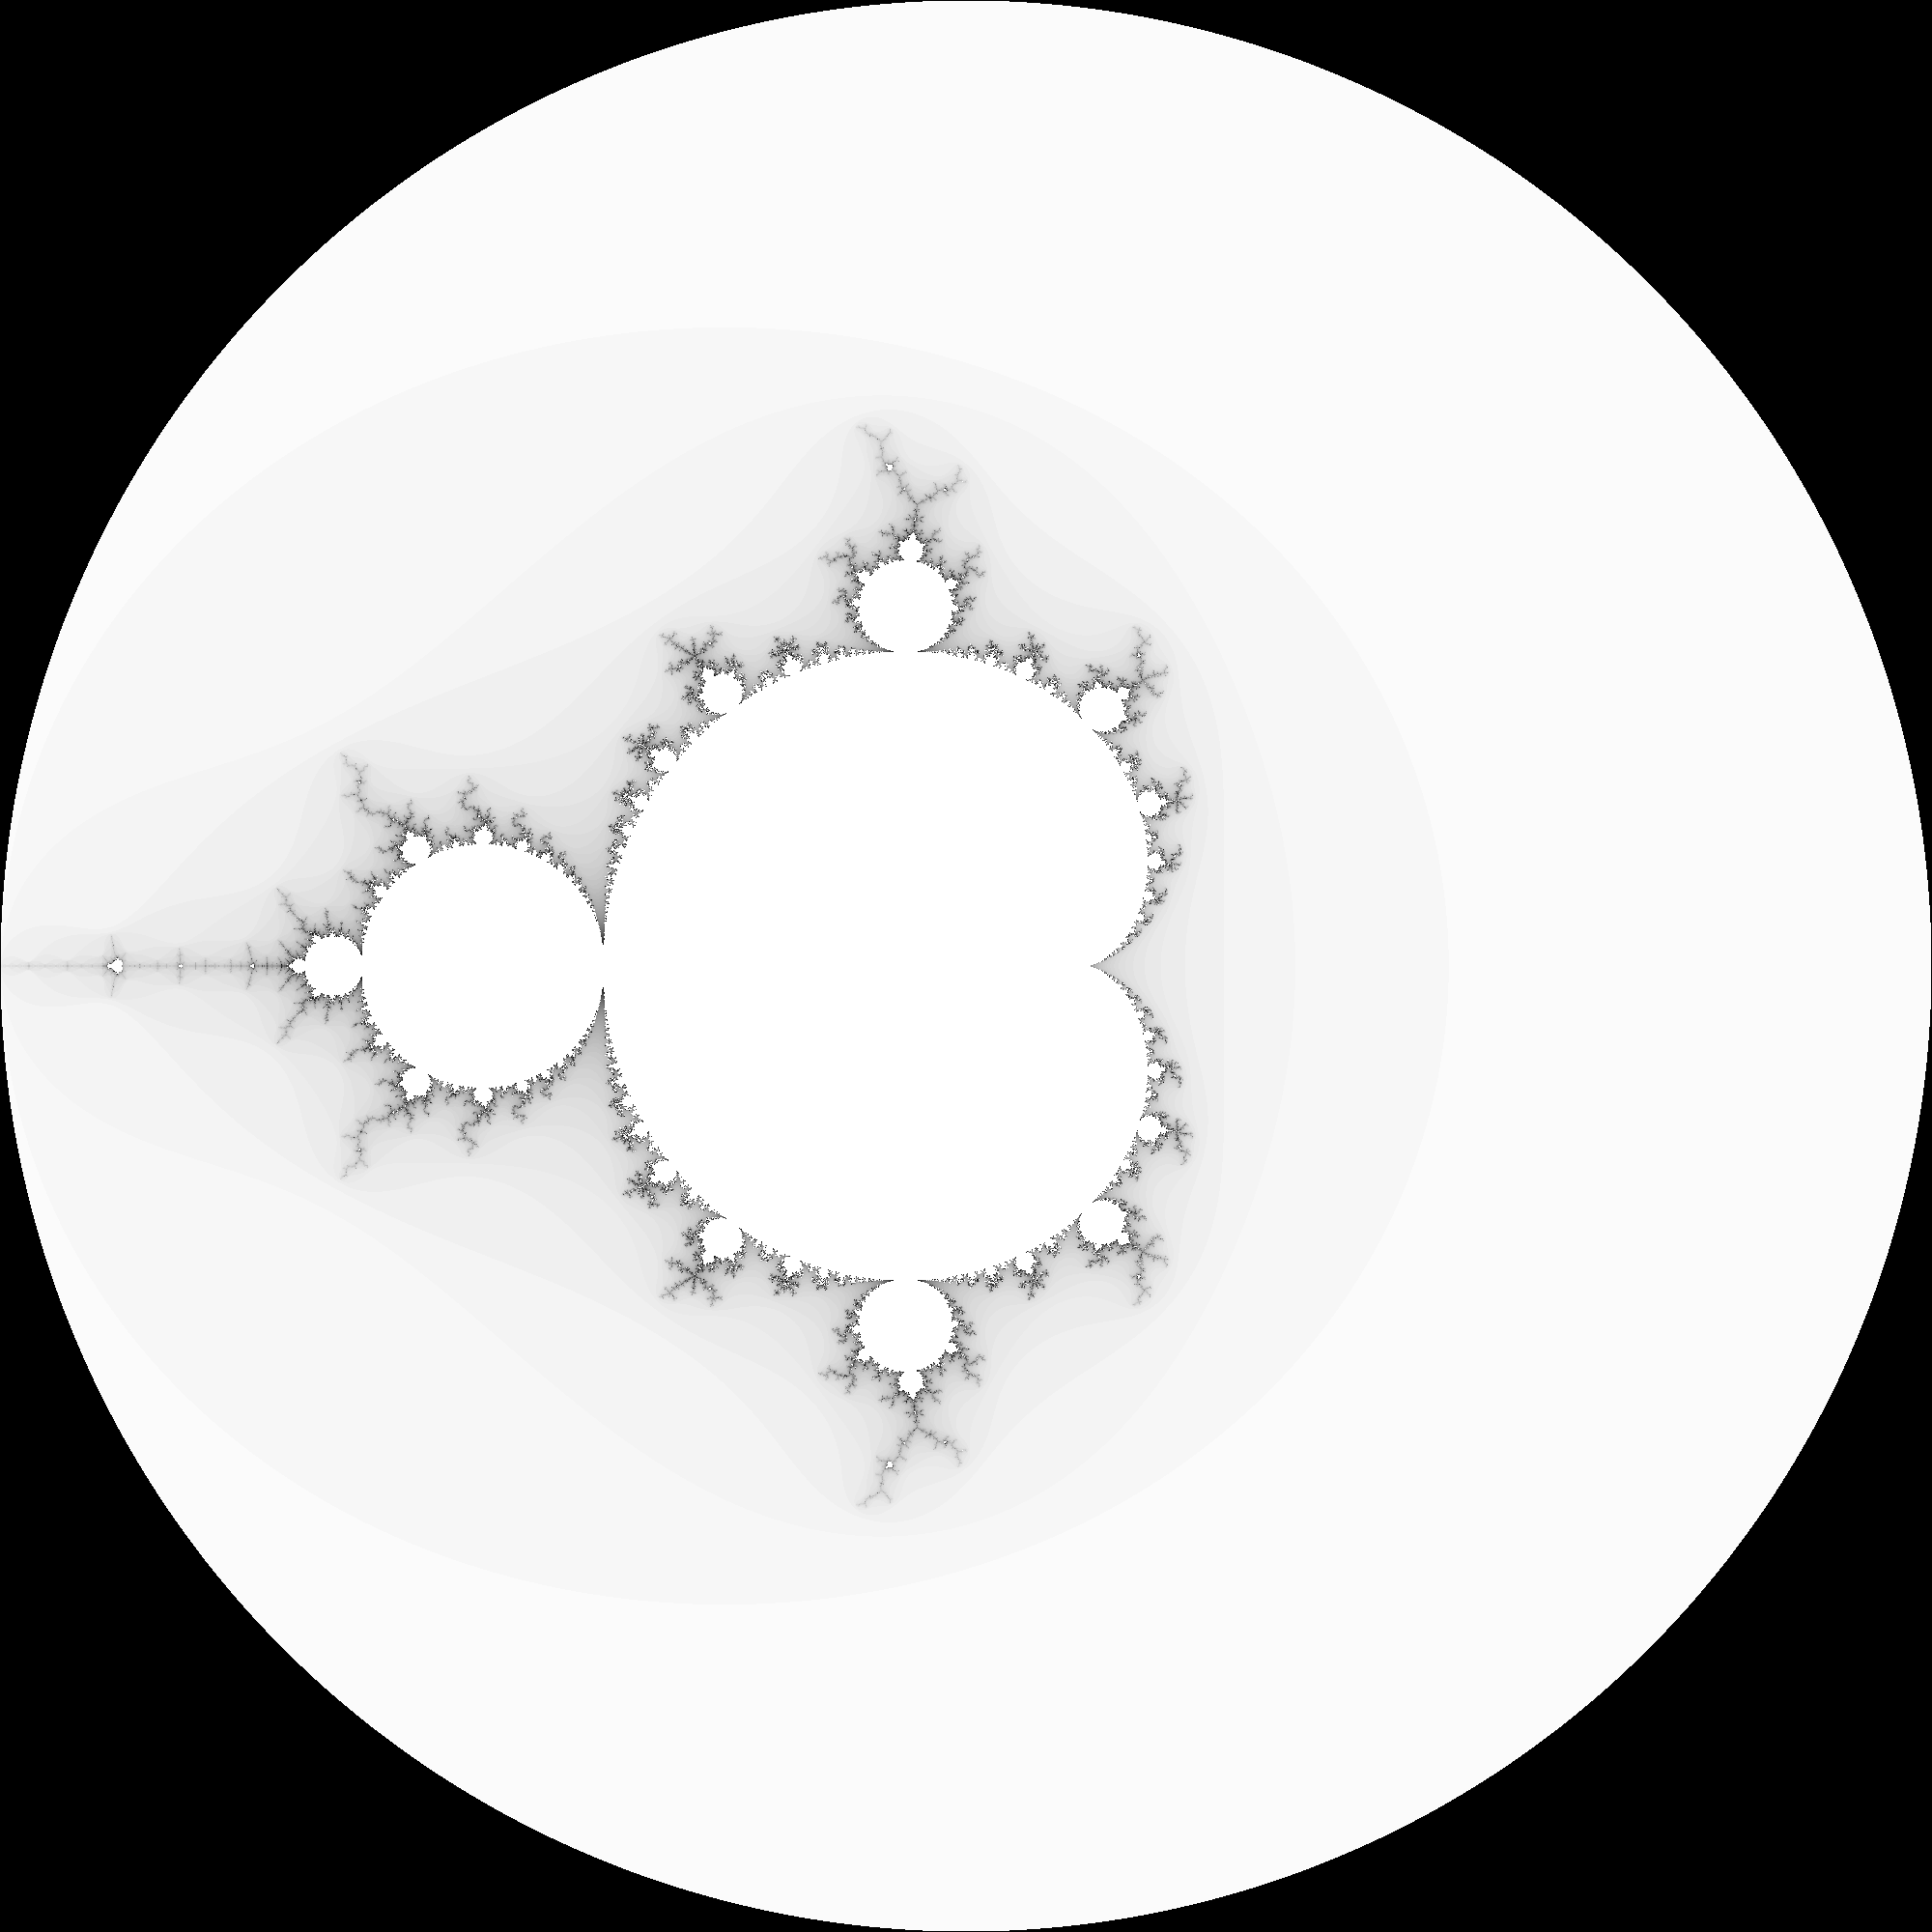
\includegraphics[width=\textwidth]{greyscale}
  \caption{
    \tiny greyscale
  }
  \label{fig:outmodegrey}
\end{subfigure}
~ %spacer
\begin{subfigure}[b]{0.3\textwidth}
  \centering
  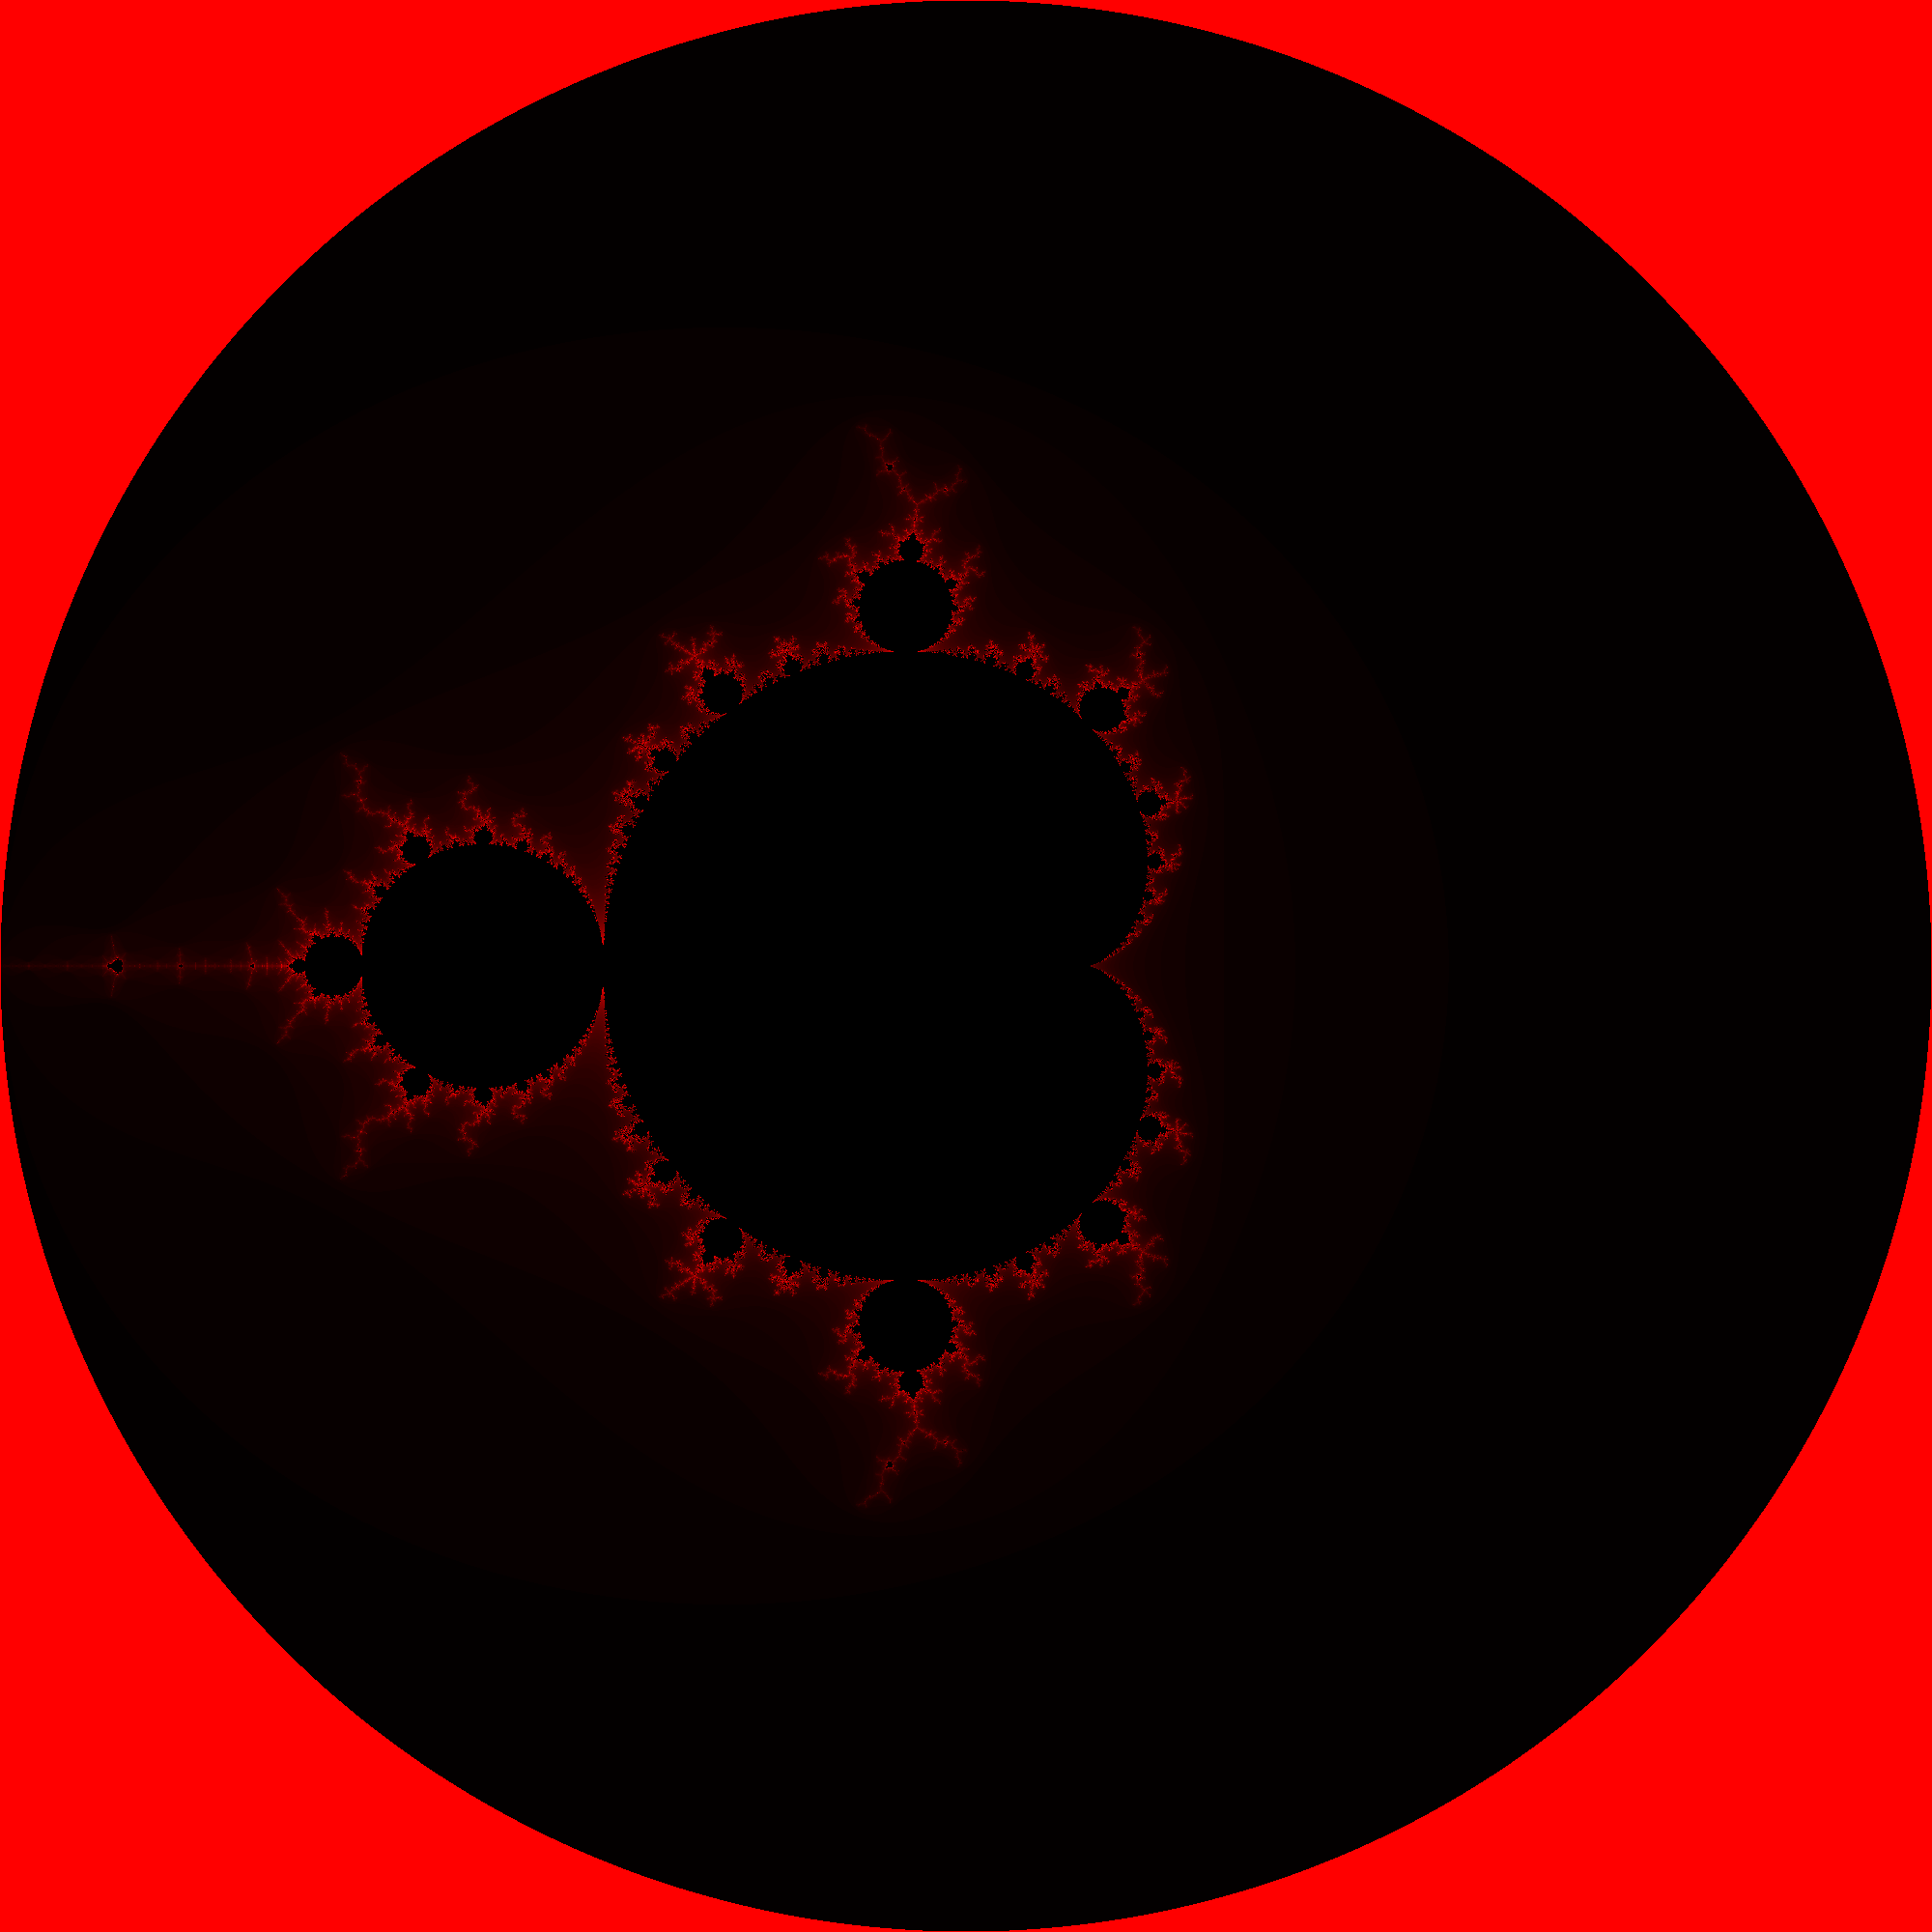
\includegraphics[width=\textwidth]{redscale}
  \caption{
    \tiny redscale
  }
  \label{fig:outmodered}
\end{subfigure}
~ %spacer
\begin{subfigure}[b]{0.3\textwidth}
  \centering
  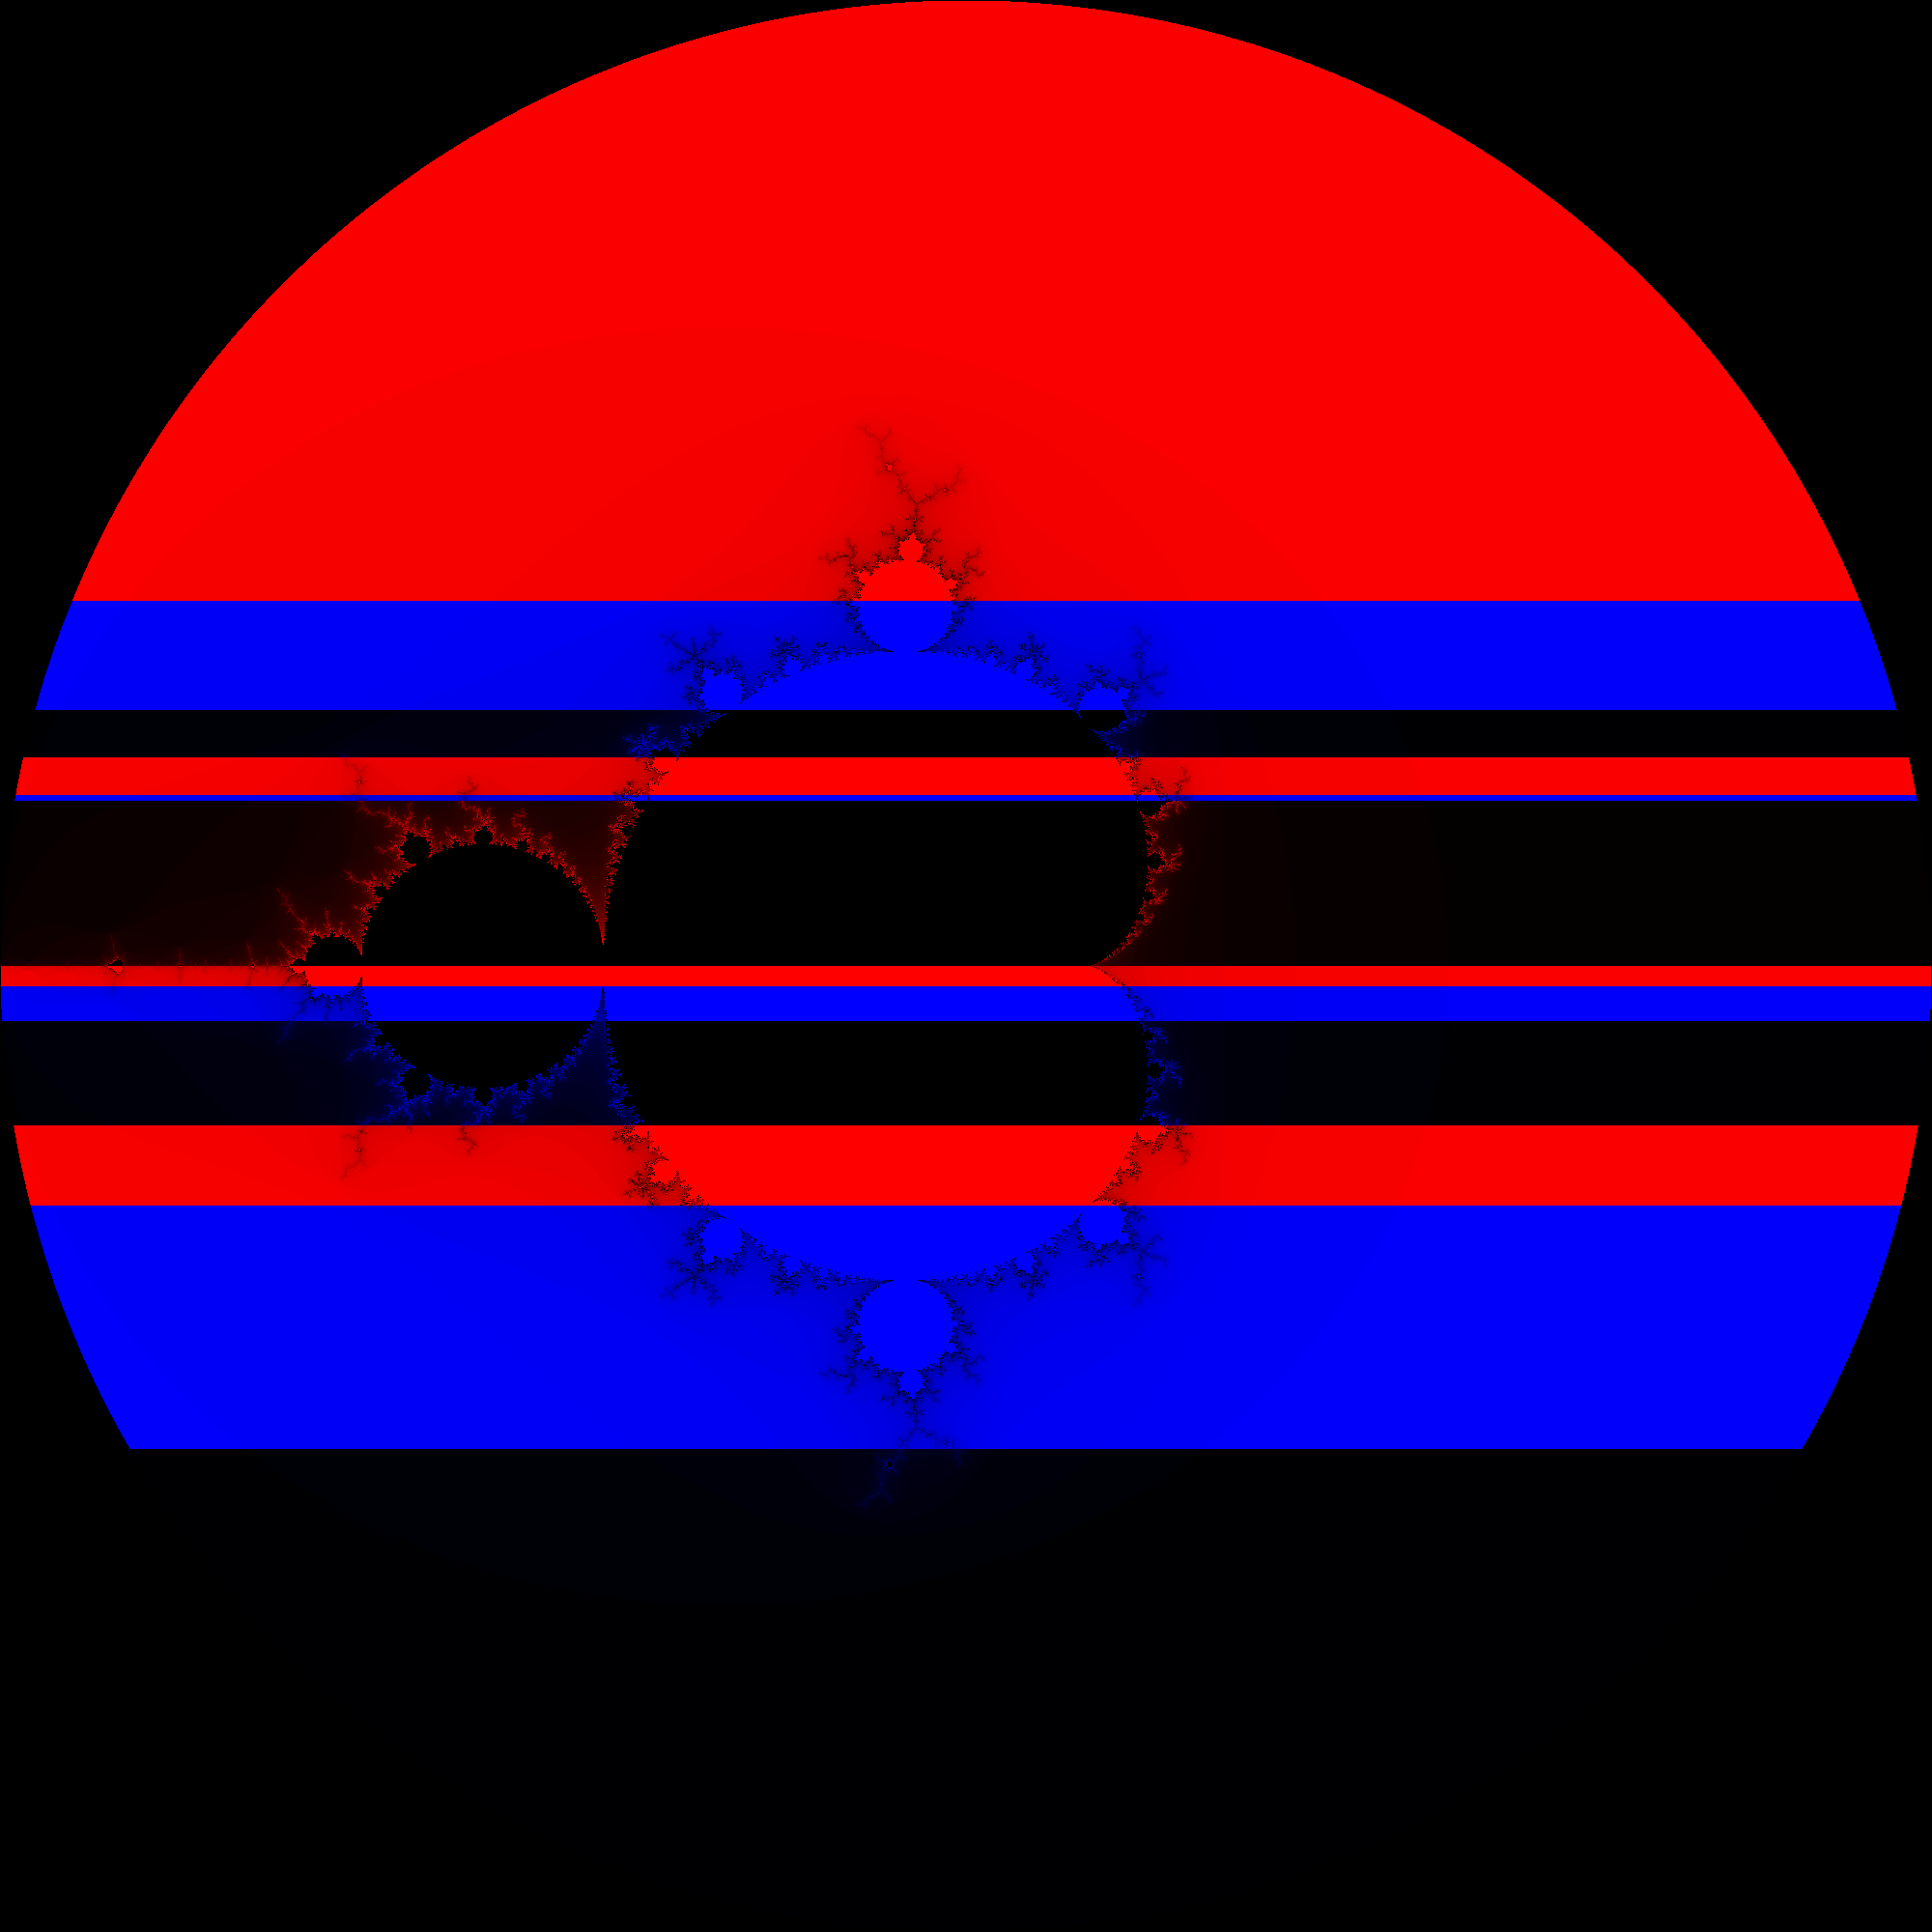
\includegraphics[width=\textwidth]{distribution}
  \caption{
    \tiny distribution
  }
  \label{fig:outmodedist}
\end{subfigure}
% full caption
\caption{
    Example images produced using the three implemented output modes. 
    All three are produced using the Randomised Work-Stealing Algorithm 
    detailed in section \ref{sec:randws}.
}
\label{fig:outmodes}
\end{figure}

